\documentclass[dvipdfmx]{jsarticle}
\usepackage[dvipdfmx]{graphicx}
\usepackage{amsmath, amssymb}
\usepackage{url}
\usepackage{mathtools}
\usepackage{here}
\begin{document}
\title{週間進捗報告}
\author{権藤陸}
\date{2022年4月20日}
\maketitle
\section{進捗}
指定していただいた論文について,分からないことを調べながら約半分まで読み進めた.
\section{論文の内容・調べたこと}
\subsection{背景・課題}
腹部表面電極から得られる非侵襲的胎児心電図(NI-FECG)は,胎児心活動の長期モニタリングを可能にすることで,出生前医療に新たな診断の可能性を提供する.しかし,NI-FECG信号は多くの干渉源,特に母体心電図(MECG)によって妨害される.

本論文執筆時点でのNI-FECGの研究の課題は2つあった.1つ目は,SNRが低い/変動するシナリオにおいて,NI-FECGの品質をどのように定量化できるか.2つ目は,誤検出を含むセグメント/チャンネルが存在する場合,複数のNI-FECGチャンネルの情報をどのように融合させることができるか,であった.
\subsection{目的}
胎児心電図のデータ推定を改善する.そのための革新的な評価指標として,新たなアルゴリズムと分類器を開発した.
\subsection{データのアノテーション}
提案手法の訓練と検証のために,大規模な注釈付き個人臨床データセットを使用した.具体的には,107人の単生児の妊婦から得られたマルチチャネルのデータ259個である.

信号品質のアノテーションについては,腹部の7チャネルから等距離の5秒間のセグメントを5つ抽出し,合計9065セグメントに対して行った.FECGの振幅は4つのクラスに,SNRレベルについては5つのクラスに分類した.また,観察者内(intra-observer)信頼性と観察者間(inter-observer)信頼性の評価のために,500セグメントのサブセットが用いられた.

胎児のQRS波に対するアノテーションは1人の専門家によって行われ,さらに2人の専門家により個々のFQRS(Fetal QRS)とMQRS(Maternal QRS)の位置が修正された.

人間による信号品質の評価のほかに,図1に示すようなSQIメトリクスを用いることで,信号品質の評価の自動化が可能である.
\begin{figure}[htbp]
\begin{center}
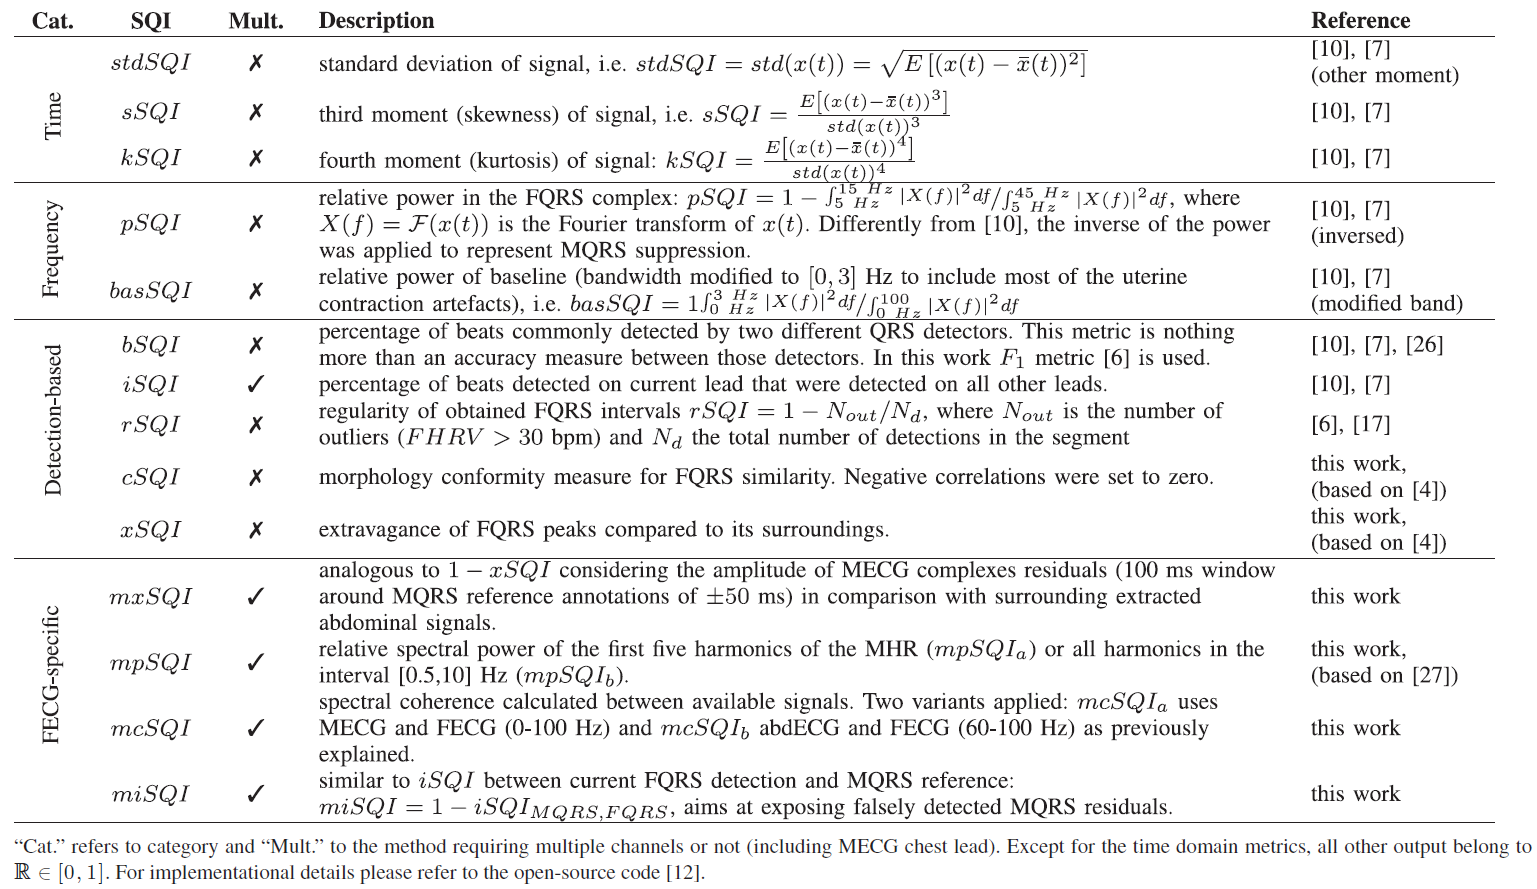
\includegraphics[width=0.9\linewidth]{./paper/sqi_metrics.png}
\end{center}
\caption{SQIメトリクスの要約}
\end{figure}
\subsection{手法}
\begin{itemize}
    \item 単純ベイズ分離器

    \noindent
    ベイズの定理から,ある結果が与えられた時の原因推定を事後確率の形で求め,その値を用いて分類を行う.シンプル故に,高速な訓練が可能という利点がある一方,各特長量が独立であるという仮定が必要となる.
    \item カルマンフィルタ

    \noindent
    時刻ごとに対象の状態推定と観測を繰り返し,複数の不確かな情報からより正確な状態を得ることを目的とする.カルマンフィルタによる状態の補正では,カルマンゲインと呼ばれる値が計算され,この値はどれだけ強く補正をかけるかを意味する.
\end{itemize}
\subsection{医学的用語}
\begin{itemize}
    \item 胸部誘導

    \noindent
    最も一般的な心電図の検査法として,定められた12方向から記録を行う12誘導心電図検査が挙げられる.その誘導法には四肢誘導と胸部誘導がある.
    \item 特異度

    \noindent
    患者が実際には病気にかかっていない場合に,検査結果が陰性になる確率.$(特異度) = (真陰性の人数) / (病気でない人数)$で表される.
    \item 黄金律 (Gold-Standard)

    \noindent
    標準基準,参照基準とも呼ばれ,診断や評価の精度が高いものとして広く容認された手法のこと.
    \item QRS complex(QRS群)
    \begin{figure}[htbp]
        \begin{center}
        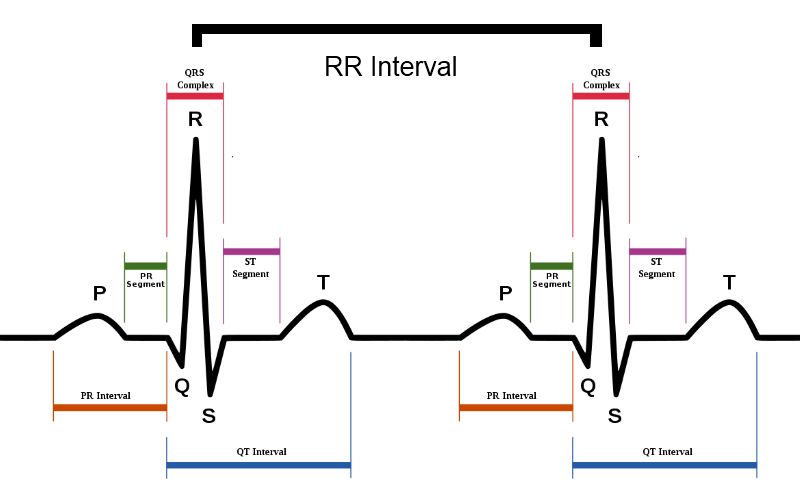
\includegraphics[width=0.85\linewidth]{./paper/The-illustration-of-QRS-complex.png}
        \end{center}
        \caption{QRS complex \cite{three}}
    \end{figure}
\end{itemize}
\section{疑問}
\begin{itemize}
    \item "\textbf{clinical acceptability}" (in \cite{one})
    \item "\textbf{false alarm reduction}" (in \cite{two})
    \item "lead"と"derivation"の違い
    \item "coherent average"
\end{itemize}
\section{今週の計画}
\begin{itemize}
    \item 解決していない疑問について調べる.
    \item 論文を読み進める.
\end{itemize}
\begin{thebibliography}{99}
\bibitem{three} ResearchGate, [Online]. 

Available:\url{https://www.researchgate.net/figure/The-illustration-of-QRS-complex_fig1_260157313}
\bibitem{one} I. Silva \textit{et al.}, “Improving the quality of ECGs collected using mobile phones: The physionet/computing in cardiology challenge 2011,” \textit{in Proc. 2011 Comput. Cardiol.}, 2011, pp. 273-276.
\bibitem{two} G. D. Clifford \textit{et al.}, “False alarm reduction in critical care,” \textit{Physiol. Meas.}, vol. 37, no. 8, pp. E5-E23, 2016.
\end{thebibliography}
\end{document}